\documentclass[a4paper,titlepage]{article}

% use this when images are included
\usepackage{float}
\usepackage{graphicx}
\graphicspath{ {./images/} }

% use for lines of code
\usepackage{listings}

% use for links, also links list of contents
\usepackage{hyperref}


\title{Digital Pen}
\date{2021\\ June}
\author{Max-Felix Müller\\ \\ 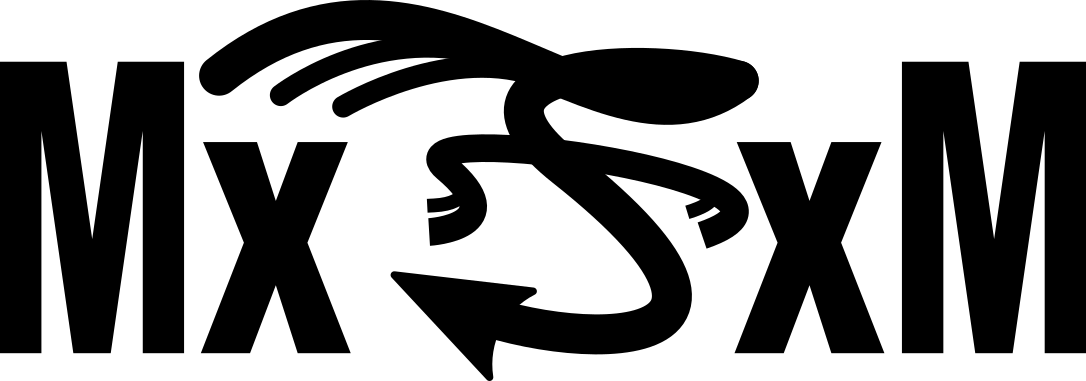
\includegraphics[width=\textwidth]{mxfxm.png}}

\begin{document}
\maketitle
\tableofcontents
\newpage
\listoffigures %delete if not necessary
\listoftables %delete if not necessary
\newpage

\section*{Abstract}

\section{First Section}
This is the first section.

\subsection{A Subsection}
Some maths. \\

$R_{1} = R_{2} = Z_{0} * \frac{N + 1}{N - 1} $\\

$R_{3} = Z_{0} * \frac{N^2 - 1}{2N} $\\

\subsection{Second Subsection}

With images...

\begin{figure}[H]
    %\includegraphics[width=\textwidth]{filename.png}
    \caption{Title of the image}
\end{figure}

\subsubsection{Subsub Section}
A line of code:

\begin{lstlisting}
    dump_errors(odrv0, True)
\end{lstlisting}

\section{Links}
\href{https://google.com}{Link to Google}

\end{document}
